\section{Network Formation Process} \label{Kap5-5}

Dieses Kapitel beschreibt im Detail den Ablauf sowie die notwendigen Funktinalit"aten
f"ur den Network Formation Process eines IEEE 802.15.4e TSCH Netzwerkes.
Dabei wird zuerst das Konzept der Enhanced Beacons
EBs zur Informationsweiterleitung beschrieben mitsamt einem beispielhaften
Minimalaufbau, bevor der Network Formation Process anhand verschiedener
Sichtweisen erl"autert wird.

\subsection{Enhanced Beacons EB}

Enhanced Beacons EBs sind anwendungsbezogene Beacons, welche auf dem
Beacon Format beruhen und werden vor allem im DSME und TSCH Mode verwendet.
Sie bilden einen Mechanismus um Informationen aus h"oheren Schichten auch auf
der MAC Schicht zu nutzen. Erkenntlich werden EBs durch das \textit{Frame Version Field}
welches den Wert \textit{0b10} bekommt. Die gesendeten Informationen werden dabei
durch die Anbindung von Information Elements IE "ubermittelt.

Im TSCH Mode werden EBs vor allem angewendet um die Synchronisation der Knoten
innerhalb des PAN sicherzustellen, sowie im Network Formation Process.

\subsubsection{Information Elements IE}
\label{subsec:IE}

Information Elements IEs sind ein bekannter Mechanismus aus dem Standard IEEE
802.11 (WLAN) und sollen Informationen auf dem MAC Sublayer transportieren,
welche vorwiegend f"ur das Management des Netzwerkes dienen.

Man kann dabei zwischen zwei Arten an IEs unterscheiden,

\begin{description}
  \item[Header IE] sind Teil des MAC Headers und liefert Informationen damit der
  Media Access Control Layer das Frame verarbeiten kann.
  \item[Payload IE] wird innerhalb des MAC Payload gesendet und soll als
  Schnittstelle zu h"oheren Schichten dienen und Informationen weitergeben.
\end{description}

Der Aufbau von IEs ist dabei in beiden F"allen identisch, er beginnt mit dem
\textit{Type Descriptor} einem Flag von 1 Bit l"ange, welcher mit 0 ein Header IE
und mit 1 ein Payload IE angibt. Dannach folgt die 8 Bit lange \textit{Element ID}
um Angaben "'uber den Inhalt anzugeben, dem \textit{Length Field} mit 7 Bit und
abschliessend den 11 Bit langen \textit{Content}.

Der exemplarische Aufbau von IEs kann in der Implementierung in \textit{lr-wpan-mac-header.cc}
ab Zeile 1270 betrachtet werden. Die Anwendung dieser und spezielle IEs, gerade
f"ur den Network Formation Process, fehlen dagegen vollst"andig und m"ussen zur
weiteren Verwendung erst implementiert werden.

\begin{lstlisting}[frame=single]
//802.15.4 IE Header
if (m_fctrlFrmVer == 2 && m_fctrlIEListPresent == 1) {
  uint8_t lastid;

  do {
    HeaderIE* newie = new HeaderIE;
    uint16_t head = i.ReadLsbtohU16 ();
    newie->length = (head >> 9); //7 bits
    newie->id = (head >> 1); //8bits
    newie->type = 0; //1bit

    for (int j = 0;j<newie->length ;j++) {
      newie->content.push_back(i.ReadU8 ());
    }
    headerie.push_back(*newie);
    lastid = newie->id;
  } while (lastid != 0x7e && lastid != 0x7f);
}

\end{lstlisting}
\subsubsection{Minimaler Aufbau eines Enhanced Beacons}
\label{sec:Aufbau_Enhanced_Beacons}
Nachfolgend ist der Aufbau eines EB dargestellt, welcher minimal notwendig
ist um die Kommunikation mittels TSCH zu gew"ahrleisten.
Das Beispiel mitsamt der Erkl"arung ist dabei dem Internet-Draft
\href{https://tools.ietf.org/pdf/draft-ietf-6tisch-minimal-12.pdf#16}{6tisch-minimal}
entnommen.

\begin{lstlisting}[frame=single]
1                   2                   3
0 1 2 3 4 5 6 7 8 9 0 1 2 3 4 5 6 7 8 9 0 1 2 3 4 5 6 7 8 9 0 1
+-+-+-+-+-+-+-+-+-+-+-+-+-+-+-+-+-+-+-+-+-+-+-+-+-+-+-+-+-+-+-+-+
| Len1 =   0  |Element ID=0x7e|0|    Len2 = 26        |GrpId=1|1|
+-+-+-+-+-+-+-+-+-+-+-+-+-+-+-+-+-+-+-+-+-+-+-+-+-+-+-+-+-+-+-+-+
| Len3 =   6    |Sub ID = 0x1a|0|           ASN
+-+-+-+-+-+-+-+-+-+-+-+-+-+-+-+-+-+-+-+-+-+-+-+-+-+-+-+-+-+-+-+-+
              ASN                               | Join Priority |
+-+-+-+-+-+-+-+-+-+-+-+-+-+-+-+-+-+-+-+-+-+-+-+-+-+-+-+-+-+-+-+-+
|  Len4 = 0x01  |Sub ID = 0x1c|0| TT ID = 0x00  |   Len5 = 0x01
+-+-+-+-+-+-+-+-+-+-+-+-+-+-+-+-+-+-+-+-+-+-+-+-+-+-+-+-+-+-+-+-+
      |ID=0x9 |1| CH ID = 0x00  | Len6 = 0x0A   |Sub ID = 0x1b|0|
+-+-+-+-+-+-+-+-+-+-+-+-+-+-+-+-+-+-+-+-+-+-+-+-+-+-+-+-+-+-+-+-+
|   #SF = 0x01  | SF ID = 0x00  |   SF LEN = 0x65 (101 slots)   |
+-+-+-+-+-+-+-+-+-+-+-+-+-+-+-+-+-+-+-+-+-+-+-+-+-+-+-+-+-+-+-+-+
| #Links = 0x01 |      SLOT OFFSET = 0x0000     |    CHANNEL
+-+-+-+-+-+-+-+-+-+-+-+-+-+-+-+-+-+-+-+-+-+-+-+-+-+-+-+-+-+-+-+-+
  OFF  = 0x0000 |Link OPT = 0x0F|         NO MAC PAYLOAD
+-+-+-+-+-+-+-+-+-+-+-+-+-+-+-+-+
\end{lstlisting}

Der Aufbau entspricht dabei dem Header IE sowie dem Payload IE eines
Enhanced Beacons.

\begin{description}
  \item[Header IE Header] Len1 = Header IE L"ange, mit dem Wert 0,
  dem Element ID 0x7e, um anzuzeigen das sofort der Payload IE anschliesst,
  sowie dem Type mit Wert 0.
  \item[Payload IE Header] der Payload IE Header gibt mit \textit{Len2} seine
  L"ange mit 26 Byte an, der \textit{GroupID} von 1, was einem MLME Header entspricht
  sowie dem Type 1.
  \item[MLME-SubIE TSCH Synchronization] f"ur die Synchronisation wird mit
  \textit{Len3} ein 6 Byte langer Payload beschrieben, \textit{SubID} gibt
  den Wert \textit{0x1a} an, was f"ur einen MLME-SubIE TSCH Synchronization Header
  wirbt. Zus"atzlich kommt der \textit{Type} Short durch den Wert 0 zur anwendung,
  sowie der \textit{Absolut Sequence Number} mit einer L"ange von 5 Byte, sowie
  der \textit{Join Priority}.
  \item[MLME-SubIE TSCH TimeSlot] beschreibt die Timeslots beginnend mit
  \textit{Len4} von 1 Byte, der \textit{SubID} mit dem Wert \textit{0x1c} der
  das IE f"ur den Timeslot (MLME-SubIE Timeslote) angibt. Dazu wird der \textit{Type}
  als Short (0) sowie der standard \textit{Timeslot template ID} von \textit{0x00}
  angegeben.
  \item[MLME-SubIE Ch. Hopping] liefert die Informationen f"ur das Channel Hopping,
  mit \textit{Len5} einer L"angenfeld von 1 Byte, der \textit{SubID} von \textit{0x09}
  welche den Header als \textit{MLME-SubIE Ch. Hopping} ausgibt, dem \textit{type}
  und seinem Wert long (1), sowie der \textit{Channel Hopping Sequence ID}.
  \item[MLME-SubIE TSCH Slotframe and Link] der letzte IE liefert schliesslich
  die Informationen "'uber das TSCH Slotframe und dem sendenen Knoten.
  Beginnen mit der L"ange in Feld \textit{Len6} von 10 Byte, der \textit{SubID}
  mit Wert \textit{0x1b} der den Anwendungsfall des IE angibt (MLME-SubIE TSCH Slotframe and Link)
  einem \textit{type} von \textit{short} (0), der \textit{Number of slotframes} mit
  \textit{0x01}, dem \textit{SlotFrame Handle} mit Wert \textit{0x00}.
  Das \textit{SlotFrame Size} Feld liefert die Gr"osse von 101 Slots an (Wert von 0x65),
  gefolgt von der \textit{Number of Links}, dem aktuellen \textit{Timeslot},
  \textit{Channel Offset} und den \textit{Link Option} der mit dem Wert \textit{0x0F}
  die Optionen \textit{tx, rx, shared} und \textit{timekeeping} angibt.

\end{description}

% ----------------------------------------
\clearpage

\subsection{Network Formation Process}

Der Network Formation Process l"asst sich dabei in zwei Bereiche aufteilen. Das
"'Werben"' (Advertising) um neue Teilnehmer f"ur das Netzwerk, durch bereits im
Netzwerk befindliche Knoten, sowie einem "'Bootstrapping"'-Verfahren das ein Knoten
durchf"uhren muss um in das Netzwerk einzutreten. In der nachfolgenden Abbildung
\ref{fig:network_formation} wird der Prozess in einem Kontrollflussgraphen dargestellt.

\begin{figure}[h]
    \centering
    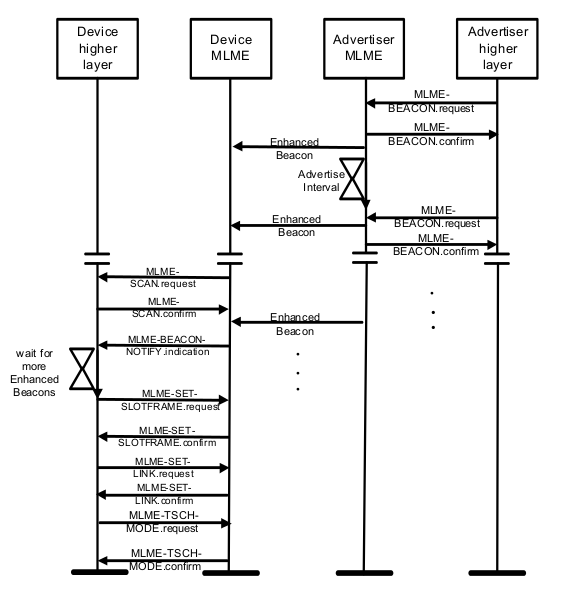
\includegraphics[scale=0.8]{images/tsch_advertisment.png}
    \caption{TSCH Prozedur f"ur Enhanced Beacons \cite{IEEE802154e}}
    \label{fig:network_formation}
\end{figure}

\clearpage
\subsubsection{Advertising}

Ein Personal Area Network PAN wird erstellt, indem ein Ger"at, in der Regel
der PAN-Coordinator die Existenz des Netzwerkes bekannt gibt. Dies geschieht
durch das Aussenden von Enhanced Beacons, welche Informationen innerhalb
von Information Elements enthalten
damit Knoten sich zum PAN synchronisieren k"onnen. Wie in Abbildung \ref{fig:network_formation}
abgebildet, beginnt das "'Werben"' indem ein \textit{MLME-BEACON.request} aus
einer h"oheren Schicht die Initiative gibt, Enhanced Beacons zu senden, welches
regelm"assig wiederholt wird.

Die enthaltenen Informationen der Enhanced Beacons, wurden konkret bereits im
vorherigen Kapitel beschrieben und enthalten:

\begin{itemize}
  \item Zeit Informationen, damit Knoten sich zum PAN synchronisieren k"onnen.
  \item Channel Hopping Informationen
  \item Timeslot Informationen, um zu erfahren wann Knoten als Receiver arbeiten
  um Frames zu empfangen und Acknowledgments zu senden.
  \item Initial Link- und Slotframe Informationen, "'ubermitteln die Informationen
  damit ein neuer Knoten weiss, wann er auf ankommende Verbindungen h"oren soll
  und wann er selber an seinen Advertisment Knoten senden kann.

\end{itemize}



Im aktuellen Entwicklungsstand wird deutlich, dass die ben"otigten IEs weder
vollst"andig implementiert sind noch deren gebrauch eingebettet ist. Als Beispiel
kann die Methode \textit{McpsDataRequest} aus dem Modul \textit{lr-wpan-tsch-mac.cc}
ab Zeile 241 gezeigt werden.

\begin{lstlisting}[frame=single]
void
LrWpanTschMac::McpsDataRequest (TschMcpsDataRequestParams params, Ptr<Packet> p)
{
...
if (params.m_frameControlOptions.IesIncluded)
  {
    macHdr.SetIEField();
    //TODO: Insert IEs
  }
else
  {
    macHdr.SetNoIEField();
  }
...
}
\end{lstlisting}

% ------------------------------------------------------------------------------
\subsubsection{"'Bootstrapping"'}

Der "'Bootstrapping"'-Algorithmus beschreibt das Verhalten von Knoten ausserhalb
des PAN und deren Aktivit"aten diesem beizutreten.

Wie in Abbildung \ref{fig:network_formation} gezeigt, wird der Knoten nach dem
Erhalt der Primitive \textit{MLME-SCAN.request} nach ankommenden EBs auf mehreren
Frequenzen suchen. Dadurch erh"alt der Knoten die notwendigen Informationen
indem er diese aus den EBs extrahiert und nun mit dem PAN sychronisiert.
Im Detail wird der Knoten sich an die Attribute der Slotframes und Timeslots anpassen,
da er sowohl die ASN wie auch die Timing-Informationen aus den IEs erhalten hat
um schlie"slich die Primitive \textit{MLME-SET-SLOTFRAME} zu aktivieren.
Anschliessend konfiguriert der Knoten seinen eigenen MLME Sublayer
mit \textit{MLME-SET-LINK} sowie dem aktivieren des TSCH Modes mit
\textit{MLME-TSCH-MODE} zur Kommunikation innerhalb des PAN.
Ist dieser Algorithmus abgeschlossen, ist der Knoten mit dem PAN innerhalb des
richtigen Slotframe und Timeslot synchronisiert und kann durch eigenst"andiges Senden
und Empfangen an diesem teilnehmen. Alle drei Primitiven sind vollst"andig im Modul
\textit{lr-wpan-tsch-mac.cc} implementiert.

\begin{itemize}
  \item MLME-SET-SLOTFRAME ist ab Zeile 1180 f"ur den Request implementiert.
    \begin{lstlisting}[frame=single]
      void
      LrWpanTschMac::MlmeSetSlotframeRequest (MlmeSetSlotframeRequestParams params)
      {
      ...
      }
    \end{lstlisting}
  \item Die Implementierung f"ur MLME-SET-LINK folgt ab Zeile 1258.
    \begin{lstlisting}[frame=single]
      void
      LrWpanTschMac::MlmeSetLinkRequest (MlmeSetLinkRequestParams params)
      {
      ...
      }
    \end{lstlisting}
  \item MLME-TSCH-MODE ab Zeile 1368 braucht noch die Abfrage der Synchronisation
    \begin{lstlisting}[frame=single]
      void
      LrWpanTschMac::MlmeTschModeRequest (MlmeTschModeRequestParams params)
      {
      ...
      }
    \end{lstlisting}
\end{itemize}
